\section{New Horizons -- Bringing the two together -- Future trends in Ocean Science}


\begin{figure}[!h]
  \centering
  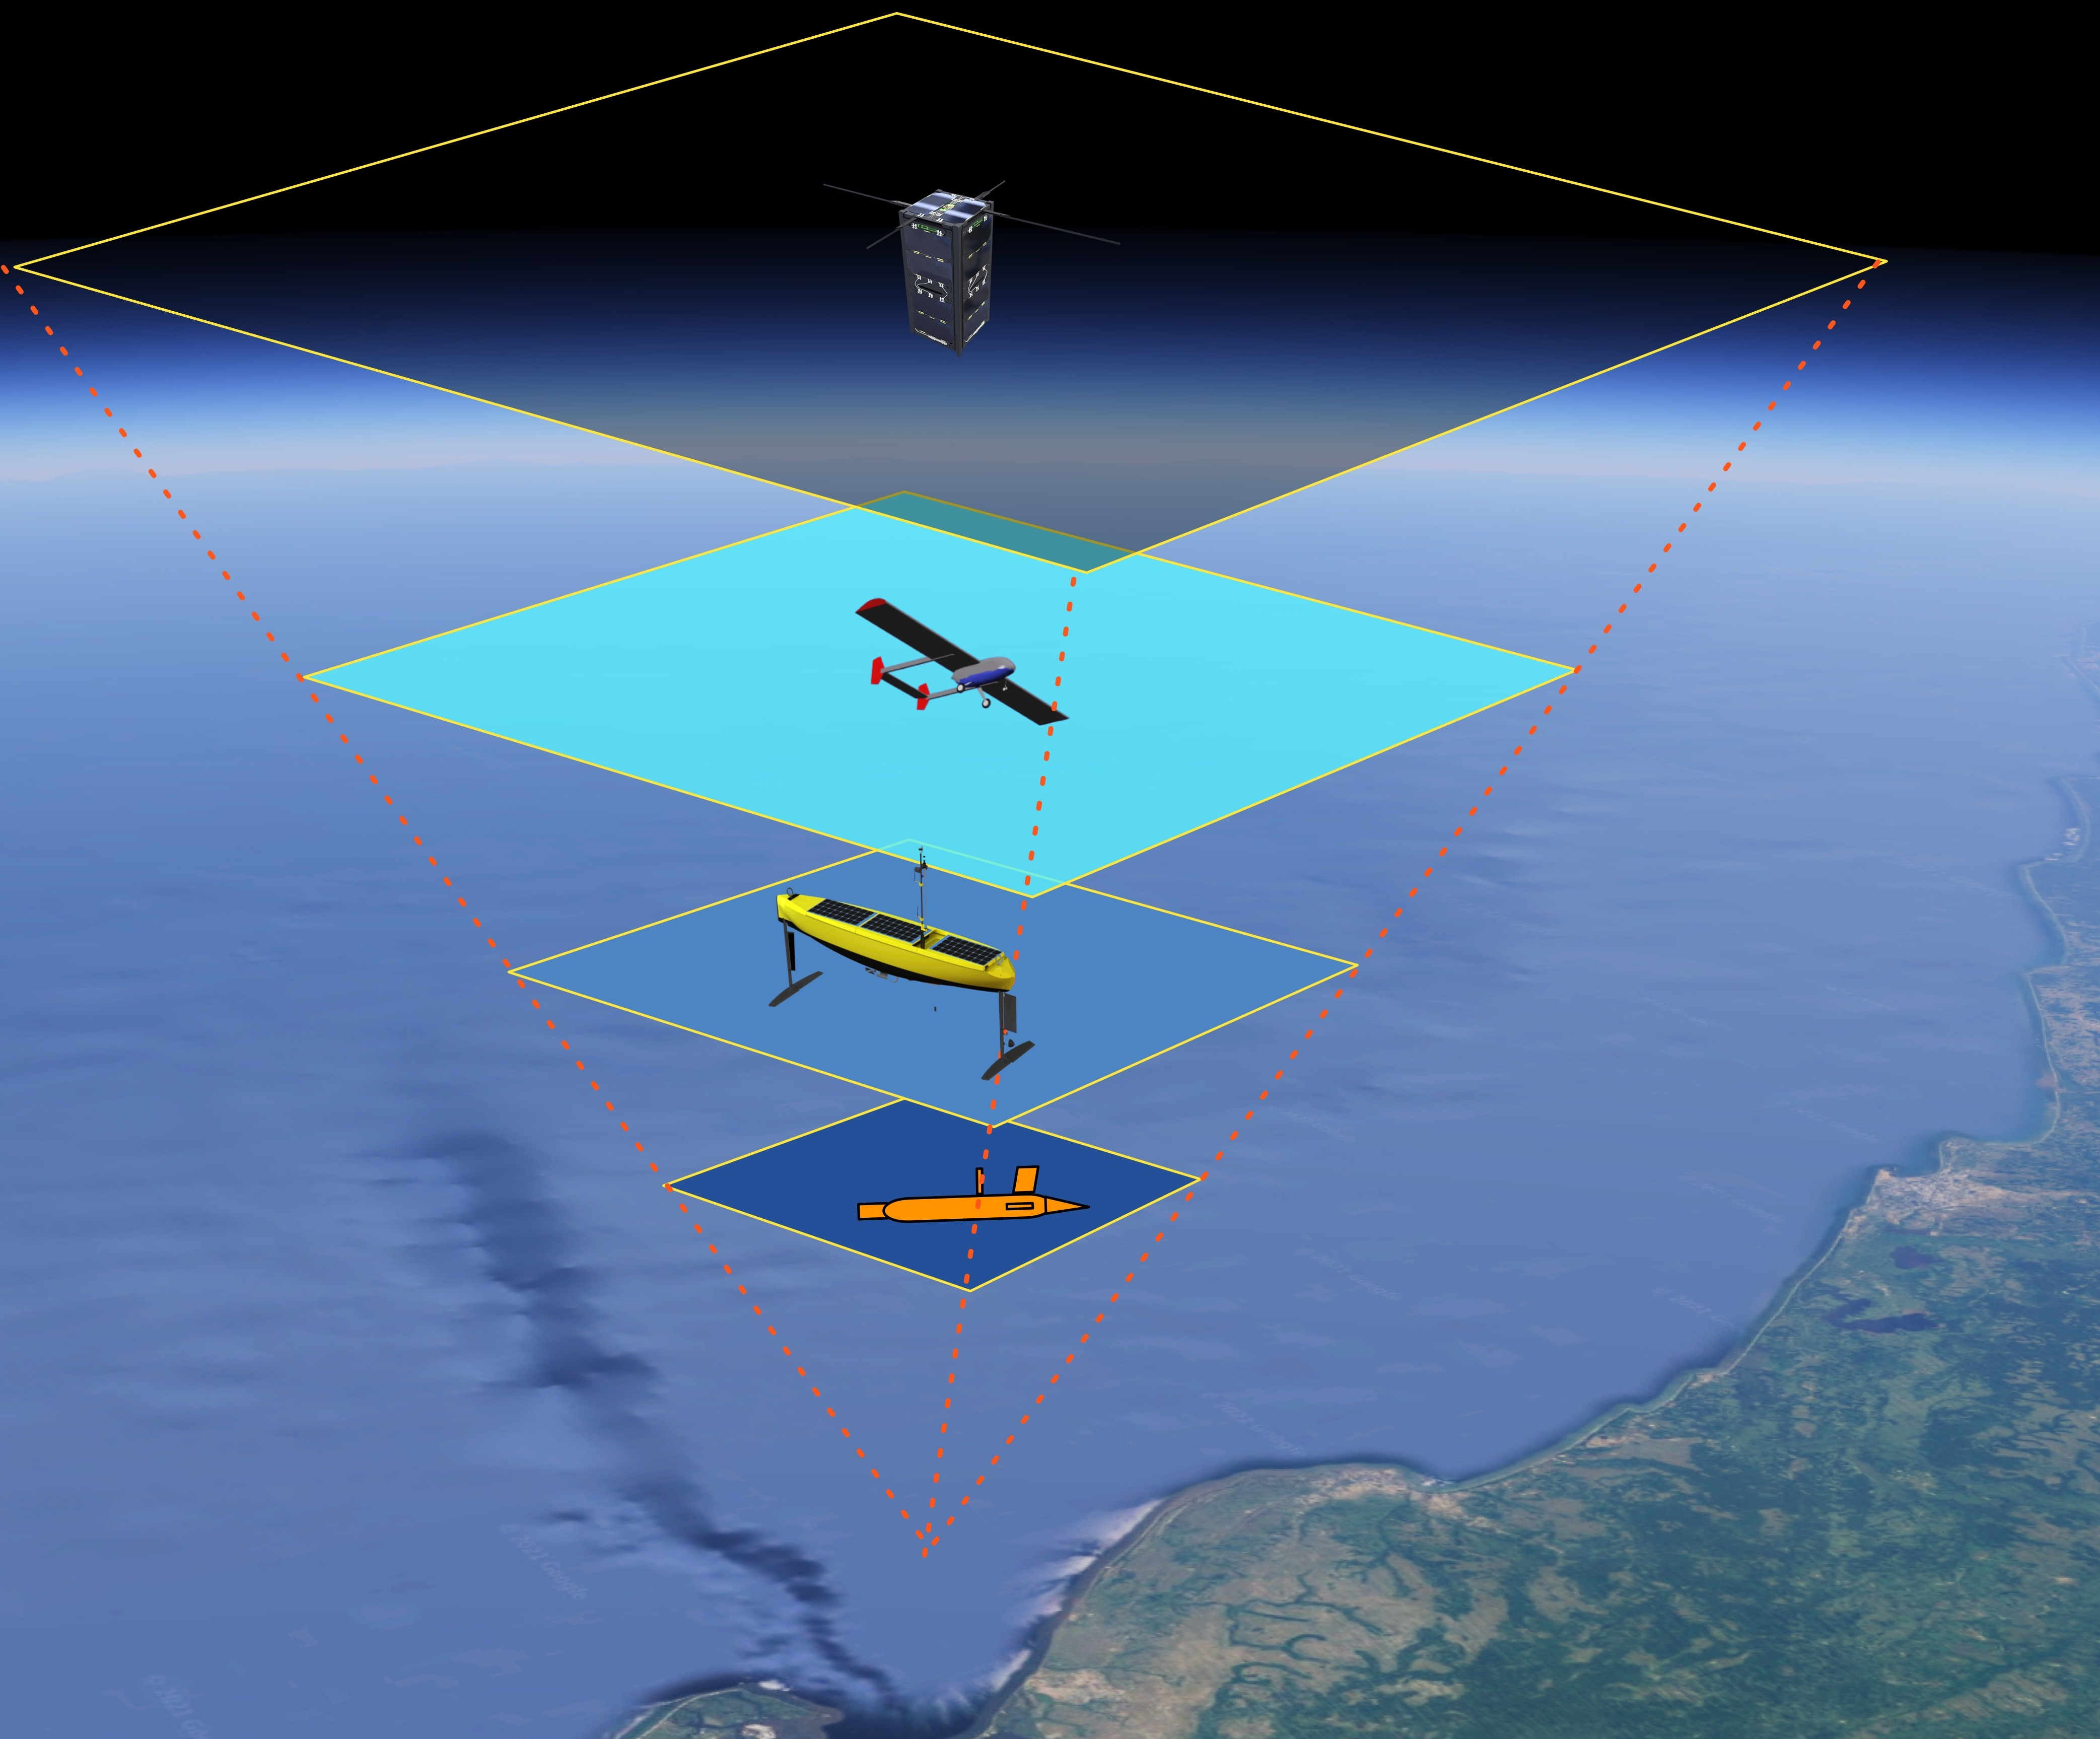
\includegraphics[width=0.9\textwidth]{fig/inverse-pyramid.jpg}
  \caption{Using multi-domain platforms from space, aerial, surface
    and underwater vehicles to observe a patch of the coastal ocean.}
  \label{fig:inverse}
\end{figure}


This could be the core of the m/s -- a look ahead to what we think the
contributions of AI and Robotics can do, leveraging networked vehicle
technologies, given large spatial extents to be sampled. 

\begin{enumerate} 

\item Implications of the use of robotic vehicles -- plusses and
  challenges. The role of vehicles in space, aerial, surface and
  underwater environments

\item how new generations of spacecraft (incl. SmallSats) could alter
  the landscape — e.g. our pitch to Audacious
  
\item How AI/ML can tie the needs of observational requirements and
  alleviate the issue of space/time and understanding spatio-temporal
  cause-effect relationships

\item The use of robots in security and surveillance. Legal implications
  related to use of robotic vehicles in such domains. 

\end{enumerate}

